\chapter{SNR G150.3+4.5}
\label{chap:G150}
Dedicated analysis  of one interesting \twofhl result. First blindly detected extended \g -ray source. 

    -Direct application of addSrcs to an intersting newly detected GeV SNR
    
    -dedicated analysis of the one source to try to understand its nature
    
    -It's interesting because :
    
    -it was blindly detected
    
    -might be the closest rem
    
    -spectrum + index seems like dynamically young, but age and distance are hard to constrain, so it could be older 
    
    -Understanding this remnant contributes to the connection between Fermi and TeV telescopes

Take this all straight from the paper I write. Not sure how much more I'd need to add
From the SNR cat, ``We also note that one classified extended candidate may be consistent with an IC origin, though no error was reported on the radio spectral index measurement by~\cite{1994MNRAS.270..106M}''. What sources is this? is G150 one of the only extended young SNRs? can't be true right? vela JR is young and extended
\section{Introduction} 
Supernova remnants have long been thought to be the primary accelerators of cosmic rays up to the knee of the cosmic ray energy spectrum. 

what to say about radio SNRs? Connect CRs to nonthermal emission and the LAT and 
Something about SNRs, cosmic ray accelerators, radio detections, connection between radio-LAT observations, G150 detection, 2FHL blind detection and SNRs at TeV (all young?), this paper extends the energy down to

Focus more on the hadronic vs leptonic since that's what's interesting? 
We describe the LAT and analysis results in $\S$\ref{sec:LATobs}, detail multiwavelength observations in $\S$\ref{sec:Multiwave}, and discuss various emission origin scenarios in $\S$\ref{sec:Discuss}.
%%%%%%%%%%%%%%%%%%%%%%%%%%%%%%%%%%%%%%%%%%%%%%%%%%%%%%%%%%%%%%%%
%
%         FermiLat  Observations and  Analysis 
%
%%%%%%%%%%%%%%%%%%%%%%%%%%%%%%%%%%%%%%%%%%%%%%%%%%%%%%%%%%%%%%%%
\section{\label{sec:LATobs}\FermiLat ~Observations and  Analysis }
\subsection{\label{sec:LATdata}Data Set and Reduction}
\FermiLat is a pair conversion telescope sensitive to high energy \gam s  from 20 MeV to greater than 1 TeV \citep{2FHL}, operating primarily in a sky-survey mode which views  the entire sky every 3 hours. The LAT has wide field of view ($\sim$2.4 sr), a large effective area of $\sim$8200 cm$^2$ above 1 GeV for on axis events and a  68\% containment radius angular resolution  of $\sim$0.8$^\circ$  at 1 GeV. For further details  on the instrument and its performance see \cite{atwood09} and \cite{lat_perf}.

In this analysis, we  analyzed 7 years of Pass 8 data, from August 2nd 2008  to August 2nd 2015. The Pass 8 event reconstruction provides a significantly improved angular resolution \jamie{this is sadly unimportant unless I'm at higher energy or using the PSF types. The P8 total PSF at 1 GeV is about the same as for P7REP. It's the acceptance/effective area that are considerably better at this energy}, acceptance, and background event rejection \citep{atwood13b,atwood13}, all of which lead to an increase in the effective energy range and sensitivity of the LAT. Source class events were analyzed within a 14$^\circ$x14$^\circ$ region centered on SNR \Gone~using the P8R2\_SOURCE\_V6 instrument response functions, with a pixel size of 0.1$^{\circ}$. To reduce contamination from earth limb \gam s, only events with zenith angle less than 100$^{\circ}$ were included.

For spectral and spatial analysis we utilized both the standard \Fermi Science Tools (version 10-01-01)\footnote[1]{\url{http://fermi.gsfc.nasa.gov/ssc/}} , and the binned maximum likelihood package \ptlike~\citep{Kerr10}. \ptlike~provides methods for simultaneously fitting the spectrum, position, and spatial extension of a source, and was extensively validated in \cite{Lande12}. Both packages fit a source model, the Galactic diffuse emission, and an isotropic component (which accounts for the background of misclassified charged particles and the extragalactic diffuse \gam~ background)\footnote[2]{\url{http://fermi.gsfc.nasa.gov/ssc/data/access/lat/BackgroundModels.html}} to the observations. In this analysis, we used the standard Galactic diffuse ring-hybrid model scaled for Pass 8 analysis, gll{\_}iem{\_}v06.fits (modulated by a power law function with free index and normalization), and for the isotropic emission,  we used iso{\_}P8R2{\_}SOURCE{\_}V6{\_}v06.txt, extrapolated to 2 TeV as in \cite{2FHL}.

In our source model for the region, we included sources from the third \FermiLat catalog \citep[3FGL]{3FGL} within 15$^\circ$ of the center of our region of interest (RoI). We replaced the position and spectrum of any 3FGL pulsars in the region with their corresponding counterpart  from the LAT 2nd pulsar catalog \citep{2PC}.  Residual emission unaccounted for by 3FGL sources is present in the RoI due to the increased time range and different energy selection with respect to that in 3FGL. We added to the RoI several point sources to account for this unmodeled emission and minimize the global residuals.\jamie{do I need to say more about these sources? should I mention adding them automatially and iteraively based on TS maps and reference SNRcat/2FHL? How close is the closest source? Mention this and use as an argument for not saying much more about them}.  The normalization and spectral index of sources within 5$^{\circ}$ of the center of the RoI were free to vary, whereas all other source parameters were fixed. A preliminary maximum likelihood fit of the RoI was performed, and  sources with a test statistic (TS) $<$ 9 (TS is defined as,  ${\rm TS}=2~{\rm Log}(\mathcal{L}_1 / \mathcal{L}_0)$ where $\mathcal{L}_1$ 
is the likelihood of source plus background and  $\mathcal{L}_0$ that of just the background) were removed from the model. 

\subsection{\label{sec:LATmorph}Morphological Analysis}
Studying the spatial extension of sources with the LAT is non-trivial due to the energy-dependent point spread function (PSF) and strong diffuse emission present in the Galactic plane. Soft spectrum point sources and uncertainties in the diffuse model can be a source of systematic error when not accurately modeling extended emission as such, particularly at low energies where the PSF is broad. To strike a balance between the best angular resolution and minimal source and diffuse contamination, we restrict our morphological analysis to energies between 1 GeV and 1 TeV. We divide this energy range into 12\jamie{4bpd} logarithmically spaced bins for both \ptlike~and \gtlike~binned likelihood analyses. 

Three  unidentified 3FGL sources are located within the extent of \Gone. 3FGL J0425.8+ 5600, located approximately 0.6$^\circ$ from the center of the SNR, is the closest of the three sources and is described with a power law spectrum of index ${\rm \Gamma = 2.35\pm 0.17}$  in the 3FGL catalog. The closest radio source to 3FGL J0425.8+5600 is NVSS J042719+560823, at 0.25° away (Ref?). 3FGL J0423.5+5442, exhibits a power law spectral index, ${\rm \Gamma = 2.63\pm 0.15}$, with no clear multiwavelength source association. Finally, 3FGL J0426.7+5437 has a pulsar-like spectrum, yet in a timing survey performed with the 100-m  Effelsberg radio telescope, \cite{Barr13} were unable to detect pulsations from the source down to a limiting flux density of $\sim$ 0.1 mJy. The source is located about 0.8$^{\circ}$ from the center of the SNR. We discuss this source and potential association with \Gone ~further in $\S$\ref{sec:Dist}). 

In our analysis, we removed 3FGL J0425.8+5600 and 3FGL J0423.5+544 from the RoI, but kept 3FGL J0426.7+5437 in the model since preliminary analyses showed clear positive residual emission at the position of the source if it was removed from the RoI. Figure \ref{fig:1GeV_resTSmap} shows a residual TS map for the region around \Gone. This point source detection-significance map was created by placing a point source modeled with a power law of photon index, $\Gamma$ = 2 at each pixel and gives the significance of detecting a point source at each location above the background. 

%put file name in {} to get it to compile with dots in the name!
%for png, have to use pdfchain
\begin{figure}[!ht]
	\begin{centering}
		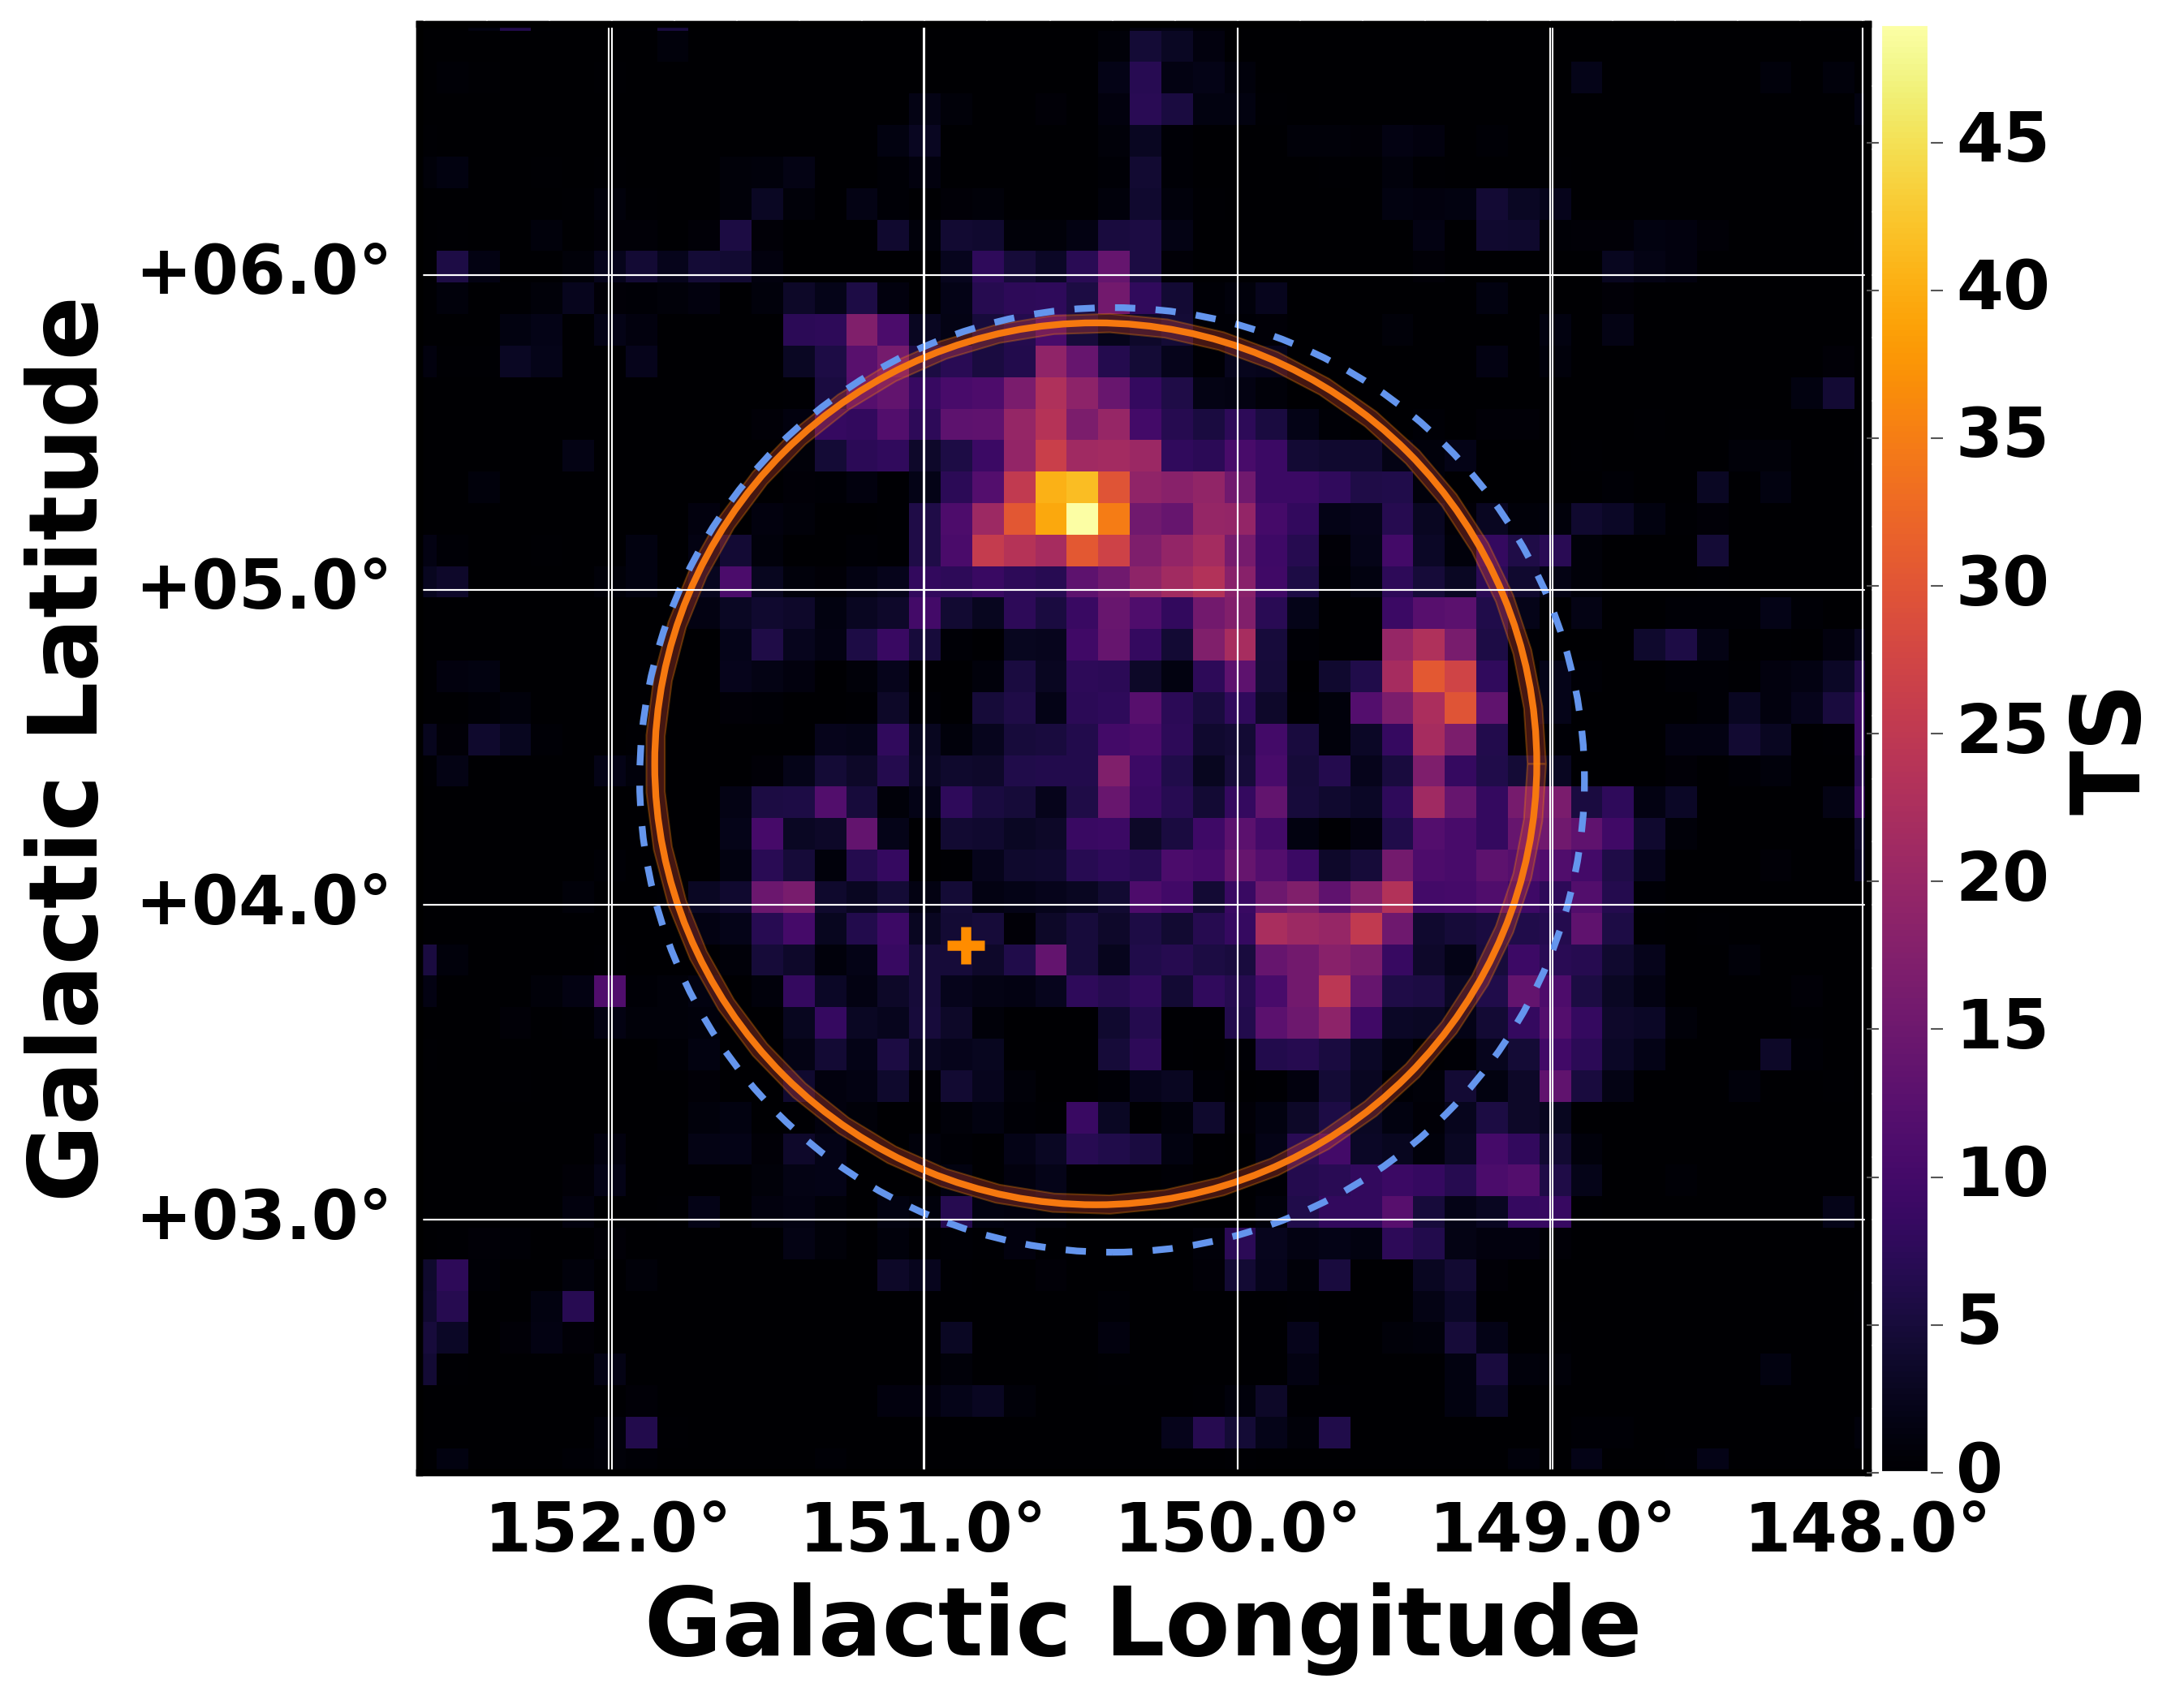
\includegraphics[width=\columnwidth]{{Figures/G150_1GeV_resTsmap_radio_noLabs}.pdf}
		\caption{Background subtracted residual TS map above 1 GeV with 0.1$^\circ$x 0.1$^\circ$ pixels for fixed index $\Gamma$ = 2, centered on SNR \Gone. The orange circle and translucent shading show the fit disk radius and 1$\sigma$ errors, respectively, for the extended source, the orange cross shows the position of 3FGL J0426.7+5437 (included in the background model), and blue dashed circle is the extent of the radio SNR. 
			\label{fig:1GeV_resTSmap}}
	\end{centering}
\end{figure}

\begin{figure}[!ht]
	\begin{centering}
		\includegraphics[width=\columnwidth]{{Figures/G150_1GeV_resTsmapNoG150_radio_noLabs}.pdf}
		\caption{Same as Figure \ref{fig:1GeV_resTSmap} but with disk in the background model \jamie{should this be a residual counts map instead?}
			\label{fig:1GeV_resTSmap_noG150}}
	\end{centering}
\end{figure}

%\begin{figure}[!ht]
%	\begin{centering}
%		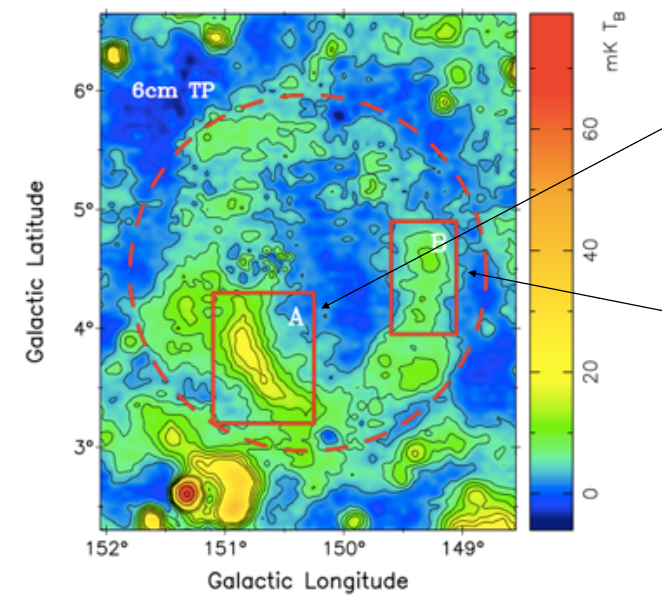
\includegraphics[width=\columnwidth]{Figures/G150_GaoHan.png}
%		\caption{This is just a filler image for now while testing things out \citep{Gao14}
%			\label{fig:GaoRad}}
%	\end{centering}
%\end{figure}

We modeled the excess emission in the direction of \Gone ~with a uniform intensity, radially-symmetric disk, simultaneously fitting the spatial and spectral components of the model  via \ptlike. The extension of the disk was initialized with a seed radius of $\sigma$ = 0.1$^\circ$ and position centered on the radio position of \Gone. We define the significance of extension as in \cite{Lande12}; ${\rm TS_{ext} = 2~log(\mathcal{L}_{ext} / \mathcal{L}_{ps})}$, with $\mathcal{L}_{ext}$ being the likelihood of the model with the extended source and $\mathcal{L}_{ps}$ that with of a point source located at the peak of emission interior to the extended source. For the disk model,  ${\rm TS_{ext} = 298}$, with a best fit radius, ${\rm \sigma = 1.40^\circ \pm 0.03^\circ}$ \jamie{I should just put this all in a table and reference it}, which is in excellent agreement with the radio size of the SNR determined in \cite{Gao14}. We tried adding back in to our model the two removed 3FGL sources but both were insignificant when fit on top of the best fit disk. Figure \ref{fig:1GeV_resTSmap_noG150} is a Residual TS map of the same region as Figure \ref{fig:1GeV_resTSmap}, but with the disk source included in the background showing that the disk can account well for the emission in the region. 

The morphology of the radio emission is suggestive of an elliptical or ring morphology, so an elliptical disk and ring spatial model were tested as well. For the ring model, the fit reduced to a disk with parameters matching those stated above. Using the elliptical model showed a weak improvement over the radially symmetric model at the 2.6$\sigma$ level (${\rm \Delta TS = 9}$ with two additional degrees of freedom), which we did not consider significant enough to say the GeV emission had an elliptical morphology (see Table \ref{tab:LATres}). For the remainder of this study, we only considered the disk spatial model.\jamie{put Edisk in table too and reference i.}
\jamie{I should double check this for 1GeV- 1TeV. I was done for 1-562 GeV, wait till addSrcs is done}



Other things we tried

fitting an extended source (starting with the 2FHL result) on top of the one currently there. Insignif. idk what to say about 2FHL yet. 

another starting at the position of G149. Insignif


Say something about why we don't just go with the 3 3FGL sources. In the table I shouldn't just compare the 3 to the disk though because I also keep J0426 in the model. So the base comparison is really 2 sources vs the disk. Maybe it's enough to just say of course we keep the disk, we find one at GeV that matches really well with the radio. What did Josh's paper say about how modelling the spectrum of an intrisically extended source as point sources skews the PS spectrum to softer energies?

He said, "Specifically, modeling a spatially extended source as point-like will systematically soften measured spectra", but idk if I get why. We see it with the 2 3FGL sources being softer than what the disk winds up being

Another thing to point out is how modeling as point vs extended, if it's really extended can affect the fit of other point sources nearby, like J0426, so I should show the spectrum of this source too?  I fit both the norm and index of the source. 
%\begin{deluxetable}{ccccccc}
\setlength{\tabcolsep}{0.04in}
\tablewidth{0pt}
\tabletypesize{\scriptsize}
\tcap{Extended Source Analysis Results\label{tab:LATres}}
\tablehead{
\colhead{Spatial Model} & 
\colhead{TS${\rm _{ext}}$} &
\colhead{TS\tablenotemark{a}} & 
\colhead{$\sigma$ [$^\circ$]} &
\colhead{R.A. [$^\circ$]} &
\colhead{DEC [$^\circ$]} & %\\
\colhead{Index}}
%\colhead{} & 
%\colhead{} & 
%\colhead{} &
%\colhead{} &
%\colhead{} &
%\colhead{}
\startdata
Disk             &    298  &     410 &  $1.40^\circ \pm 0.03^\circ$  & $55.46^\circ \pm 0.03^\circ$          & $66.91^\circ \pm 0.03^\circ$ & $1.82 \pm 0.04$  \\
Elliptical Disk  &    189.048 &   34 &  $1.78^\circ / 1.23^\circ \pm 0.02^\circ$  & $66.61^\circ \pm 0.04^\circ$ & $55.43^\circ \ pm 0.03^\circ$   & $1.86 \pm 0.04$ \\
2FHL (free)\tablenotemark{b}  &    260.317 &     17  &  $0.80^\circ \pm 0.04^\circ$  & $69.33^\circ \pm 0.06^\circ$      & $56.00^\circ \pm 0.06^\circ$ & $1.34 \pm 0.17$   \\
2FHL (fixed) &    260.317 &     -3.277  &  63.87  & Puppis A      & snr    & 1.4\\
Disk \& 2FHL\tablenotemark{b}     & 4 &     17  &  $0.80^\circ \pm 0.04^\circ$  & $69.33^\circ \pm 0.06^\circ$      & $56.00^\circ \pm 0.06^\circ$ & $1.34 \pm 0.17$   \\

%\cutinhead{Thee Point Sources}
%\sidehead{Uniform Disk}
\enddata
\tablecomments{~ 2FHL (free) corresonds to the model where a disk matching \ghard{}, was included in the likelihood model and the spectral and spatial parameters we free to vary. For the 2FHL (fixed) model, \ghard{} was included with spatial parameters fixed. In the Disk \& 2FHL model, we included both the best-fit disk determined in $\S$\ref{sec:LATmorph}, fixed in position and size, and added a source resembling the \ghard{} with free spectral and spatial parameters. This model reports the fit values of \ghard{}
 }

\tablenotetext{a}{Calculated in \gtlike}
\tablenotetext{b}{Started with disk matching the spectral/spatial parameters of \ghard{}, then left them free to fit in the likelihood model.}
\end{deluxetable}




                



\subsection{\label{sec:LATspec}Spectral Analysis}
After determining the best fit morphology with \ptlike~for the GeV emission coincident with SNR \Gone, we used those results as a starting point for our \gtlike~maximum likelihood fit of the region to estimate the best spectral parameters for our model. The LAT data is well described by a power law across the entire energy range with a photon index, ${\rm \Gamma = 1.80 \pm 0.04}$, and energy flux above 1 GeV of ${\rm (7.17 \pm 0.73~ x 10^{-11})~ erg~cm^{-2}~ s^{-1}}$and TS = 373 \jamie{these are the pointlike results, change them when I get the gtlike res}. We tested the \gam ~spectrum of the extended disk for spectral curvature using a log-normal model (Log Parabola), and find no significant deviation from a power law (${\rm \Delta TS \sim 1}$). 

\begin{figure}[!ht]
	\begin{centering}
		\includegraphics[width=\columnwidth]{Figures/{G150.3+4.5_SED}.png}
		\caption{Spectral energy distribution for the extended source coincident with SNR \Gone. \jamie{replace with gtlike SED when I have it}
			\label{fig:G150SED}}
	\end{centering}
\end{figure}

\begin{figure}[!ht]
	\begin{centering}
		\includegraphics[width=\columnwidth]{Figures/{G150.3+4.5_3FGLJ0426.7+5437_SED}.png}
		\caption{Spectral energy distribution of 3FGL J0426.. \jamie{replace with gtlike SED when I have it}
			\label{fig:J0426SED}}
	\end{centering}
\end{figure}
Still to do

gtlike


Systematics. Bracketing IRFs, alt iem, try varying the extension? still need to be done. Should probably just move this into the spectral  section


%%%%%%%%%%%%%%%%%%%%%%%%%%%%%%%%%%%%%%%%%%%%%%%%%%%%%%%%%%%%%%%%
%
%         Multiwavelength  Observations and  Analysis 
%
%%%%%%%%%%%%%%%%%%%%%%%%%%%%%%%%%%%%%%%%%%%%%%%%%%%%%%%%%%%%%%%%

\section{\label{sec:Multiwave}Multiwavelength  Observations and  Analysis }
\subsection{\label{sec:HI}HI}
\subsection{\label{sec:CO}CO?}
Do the CO maps add anything?
\subsection{\label{sec:Xray}X-ray}
No diffuse nonthermal X-ray emission observed by ROSAT. No point sources near the center? Should a  pulsar even  be near the center? How to quantify this? Can we place a limit on ambient density with an upper limit on thermal X-ray emission? Magnetic filed with nonthermal?

%%%%%%%%%%%%%%%%%%%%%%%%%%%%%%%%%%%%%%%%%%%%%%%%%%%%%%%%%%%%%%%%
%
%         Discussion and Results
%
%%%%%%%%%%%%%%%%%%%%%%%%%%%%%%%%%%%%%%%%%%%%%%%%%%%%%%%%%%%%%%%%
\section{\label{sec:Discuss}Discussion and Results}
\subsection{\label{sec:What}What is it?}
Size + HI suggest that near distance corresponding to different HI velocities suggest it's aged, spectrum looks more like young SNR (hard + no GeV break ). Is it a weird young remnant or weird aged one? Leptonic dominated if young, hadronic dominated if older? Something about nearby dense clouds masking hadronic emission? Maybe this is only true for MeV cosmic rays that are screened out though and it would only mask the pion bump, but not this higher energy emission?

PWN or SNR. Can we rule out PWN? See W41 paper, MSH 11-61A, Fabios recent G326 work (no, he just tries to use the PSF types and testing different model templates to try to disentangle SNR from PWN)?

No PSR candidate near center (should it be near the center? Depends on age)
Is there some limit we can place on the PWN based on not seeing the pulsar? Like on Edot? OR something like Mattana et al. 2009 correlation between  $\mathrm{flux_x / flux_g \propto}$   Edot? 

Assume it's in Sedov phase based on size + near distance, and calculate age, upper limit on Edot base on lack of x-ray flux? Or maybe if I assume the sources is the PWN and GeV radius is PWN radius, then can I estimate Edot based on size and evolution inside  SNR?

If we assume close distance, age is only $\approx$ 5kyr, maybe this is a transitional SNR? What do others like this look like? Puppis A? Gamma Cygni is a similar age too.something 


\subsection{\label{sec:Dist}Distance Considerations}
probably doesn't need to be a different section. 
\subsection{\label{secModel}Nonthermal Modeling}
I think I could get a working model with naima running pretty quickly, is it worth it?
%%%%%%%%%%%%%%%%%%%%%%%%%%%%%%%%%%%%%%%%%%%%%%%%%%%%%%%%%%%%%%%%
%
%         Conclusion
%
%%%%%%%%%%%%%%%%%%%%%%%%%%%%%%%%%%%%%%%%%%%%%%%%%%%%%%%%%%%%%%%%
\section{\label{sec:Conc}Conclusions}
\jamie{most of this should be the conclusions from the G150 paper}In this chapter, we have presented the publication on the dedicated analysis of the extended \g -ray emission detected in the direction of \Gone. \Gone ~was first detected in radio by \cite{Gao14}, and subsequently detected in \g-rays in \twofhl above 50 \gev. We discussed our \lat morphological analysis at energies E $\geq$ x \gev~and spectral analysis down to E $\geq$ 750 \mev, demonstrating a change in extension and centroid position compared to the \twofhl result. Discuss potential source origin scenarios. Is it SNR or PWN? Is \twofhl source same as $>$ few \gev? 

\jamie{for diss, not paper}. The way this figures into the whole is that  this is a follow up analysis of one of the most interesting  sources detected with addSrcs, and, (hopefully!), we're able to say something about the source and nature of the \g-ray emission, relation to SNR and \twofhl source1